\section{Results}
\label{sec:results}

We start by describing the results for each study in detail, before proceeding to summarize and discuss the observed effects.

\subsection{Experimental Simulation}
\label{sec:expResults}

%demographics
The selected participant set encompasses graduates in Computer Science or Software Engineering -- either working in industry (41.6\%) or M.Sc. and Ph.D. candidates (58.4\%).
%table
In Table~\ref{tab:results} we summarize the results from the 24 trials, from which five -- 21\% -- were delivered with at least one fault detected by our test cases.
%individual results
All participants assigned to textual specifications in Javadoc delivered correct programs.
By contrast, half of the programs delivered by participants using APIs with formal contracts were faulty (four out of eight).
One faulty program was delivered by a participant from the \contractjdoc{} group.
%task
Regarding task, faulty programs were mostly present in implementing in API implementations -- four of them, if compared with only one in API clients.


% source code correct
%Javadoc and \contractjdoc{} were the only documenting approaches in which all participants were able to produce a code satisfying the oracle (respecting the restrictions available in the comments). On the other hand, there was one case developed by following the JML documenting approach in which the contract is not satisfied by the implementation.



\begin{table}
\centering
\caption{Experimental results, for each treatment (textual Javadoc \emph{JavaDoc}, \contractjdoc{} \emph{ContJDoc} and formal contracts \emph{Formal}. For each API (Queue or Stack) and Task (\emph{Cli} if a client for the API was implemented, \emph{Sup} if an implementation for the API was provided), participants are listed (\emph{Part}) along with the result (\emph{Res}) from our test cases.}
\label{tab:results}
\begin{tabular}{|l|l||l|l||l|l||l|l|} 
\cline{3-8}
\multicolumn{1}{l}{} &              & \multicolumn{2}{l||}{\textbf{JavaDoc }} & \multicolumn{2}{l||}{\textbf{ContJDoc }} & \multicolumn{2}{l|}{\textbf{Formal}}  \\ 
\hline
\uline{DataStr}      & \uline{Task} & Part & Res                              & Part & Res                                & Part & Res                             \\ 
\hline\hline
\uline{Queue}        & \uline{Cli}  & p9   & \greencheck       & p11  & \greencheck                                    & p7   & \greencheck                                 \\
                     & \uline{Cli}  & p10  & \greencheck                                 & p12  & \greencheck                                    & p8   & \greencheck                                \\
                     & \uline{Sup}  & p21  & \greencheck                                 & p23  & \greencheck                                    & p19  &  \greencheck                               \\
                     & \uline{Sup}  & p22  & \greencheck                                 & p24  & \greencheck                                    & p20  &  \redcross                               \\ 
\hline\hline
\uline{Stack}        & \uline{Cli}  & p3   & \greencheck                                 & p5   & \greencheck                                    & p1   & \redcross                                 \\
                     & \uline{Cli}  & p4   & \greencheck                                 & p6   & \greencheck                                    & p2   & \greencheck                                 \\
                     & \uline{Sup}  & p15  & \greencheck                                 & p17  & \redcross                                    & p13  & \redcross                                \\
                     & \uline{Sup}  & p16  & \greencheck                                 & p18  & \greencheck                                    & p14  & \redcross                                \\
\hline
\end{tabular}
\end{table}

%faults
Table~\ref{tab:faults} details the faults detected by the test cases. After detailed analysis of the programs, we classified each fault in terms of the violated contract. 
%clients
All clients fulfilled the specified pre-conditions for calling the API methods -- p1's API client raise an exception which was incompatible with the method's postcondition.
%suppliers
All four faults unveiled in API implementations resulted from failure in satisfying the specified post-condition in methods removing data from the given structure (two on \texttt{Stack.pop} and two on \texttt{Queue.remove}).

\begin{table}
\centering
\caption{Reason (fault) for failures in participants' results}
\label{tab:faults}
\begin{adjustbox}{width=\textwidth}
\begin{tabular}{|l|l|l|l|} 
\hline
\multicolumn{4}{|l|}{\textbf{ContractJDoc }}                                                                                                                                                                    \\ 
\hline
p17                                        & Stack                             & Sup                                & Post-condition violation on method \texttt{remove}                                    \\ 
\hline
\multicolumn{4}{|l|}{\textbf{Formal contracts} }                                                                                                                                                                \\ 
\hline
p1                                         & Stack                             & Cli                                & Failure to expect correct exceptions from Post-condition on method \texttt{removeAccountTop}    \\ 
\hline
p13                                        & Stack                             & Sup                                & Post-condition violation on method \texttt{pop}     \\ 
\hline
p14                                        & Stack                             & Sup                                & Post-condition violation on method \texttt{pop}     \\ 
\hline
p20                                        & Queue                             & Sup                                & Post-condition violation on method \texttt{remove}  \\ 
\hline\hline
\multicolumn{1}{|c|}{\textbf{Part}} & \multicolumn{1}{c|}{\textbf{API}} & \multicolumn{1}{c|}{\textbf{Task}} & \multicolumn{1}{c|}{\textbf{Type of~Fault}}                                               \\
\hline
\end{tabular}
\end{adjustbox}
\end{table}

After they sent their code back, we asked participants about understandability of the API specifications, using a Likert-like scale which ranges from 1 (less understandable) to 5 (very understandable). The results for 24 answers are summarized in Figure~\ref{fig:ExpAnswersTotal}, where we can see assessments are split between 3 to 5. Most participants evaluated understandability as 4 (58\%).

\begin{figure*}
\centering
\begin{subfigure}{.32\textwidth}
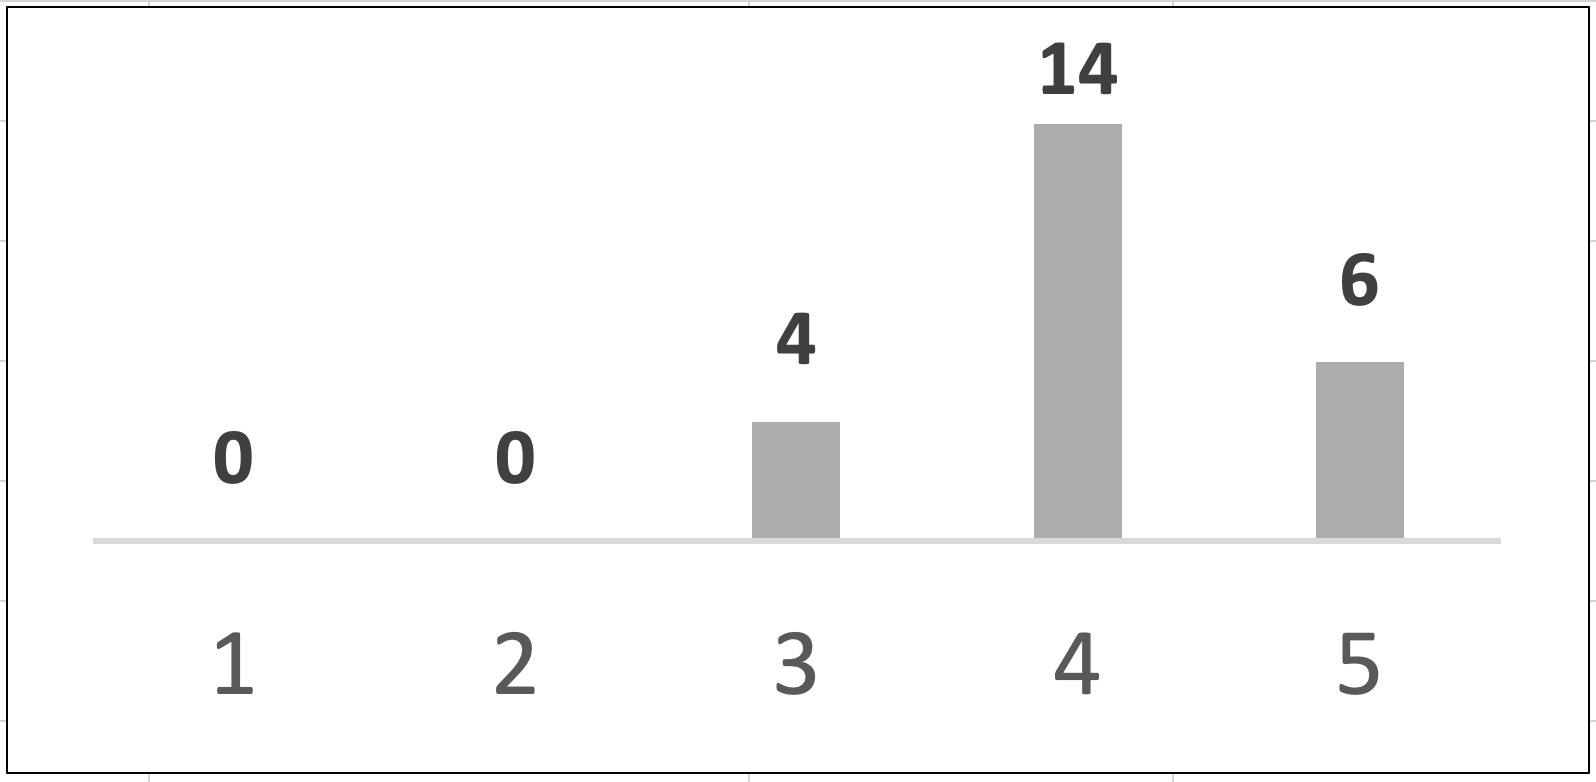
\includegraphics[width=1\textwidth]{figs/ExpAnswersTotal.png}
\caption{Total Results.}
\label{fig:ExpAnswersTotal}
\end{subfigure}
\begin{subfigure}{.33\textwidth}
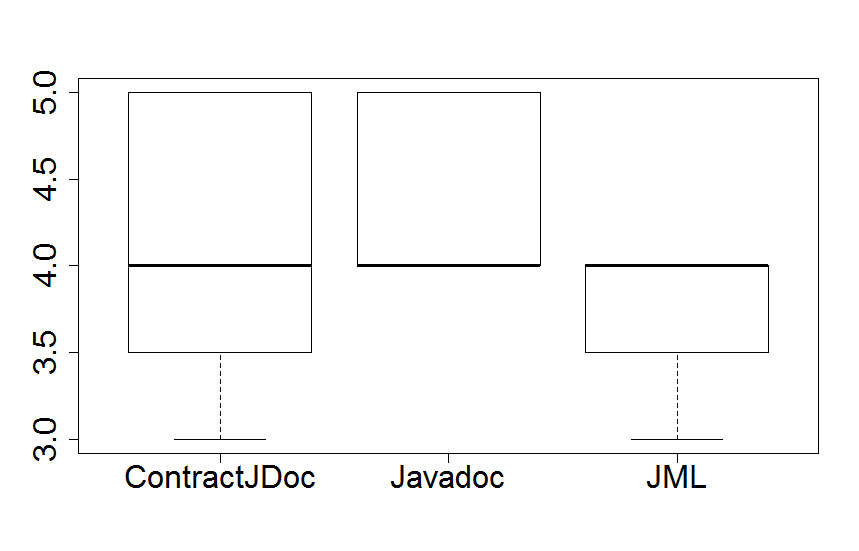
\includegraphics[width=1\linewidth]{figs/boxplotApproachesEmpiricalStudy}
\caption{Results by approach.}
\label{fig:approachesEmpirical}
\end{subfigure}
\begin{subfigure}{.33\textwidth}
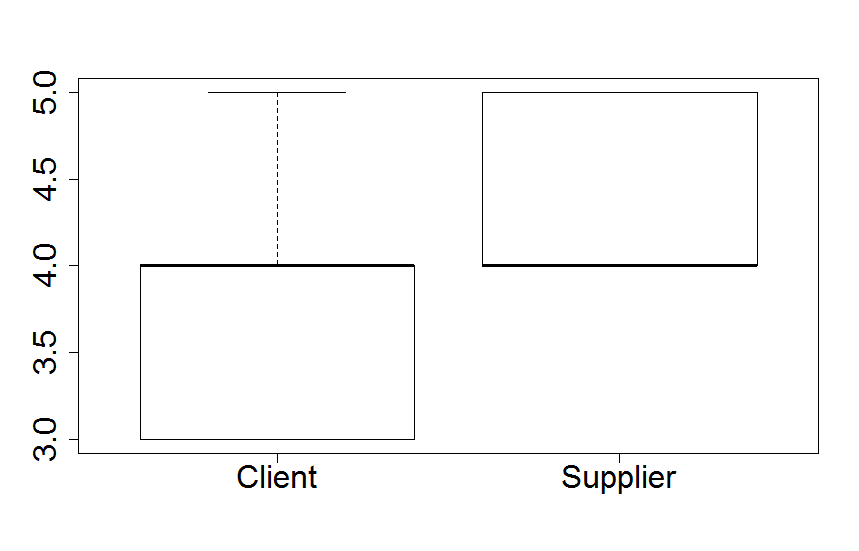
\includegraphics[width=1\linewidth]{figs/boxplotTasksEmpiricalStudy}
\caption{Results by task.}
\label{fig:tasksEmpirical}
\end{subfigure}
\caption{Results from Understandability Assessment of API specifications, as Perceived from Participants.}
\label{fig:empiricalResults}
\end{figure*}

%perspectives
Assuming a distinct perspective, we grouped understandability assessments by the assigned documentation approach and task -- Figures~\ref{fig:approachesEmpirical} and~\ref{fig:tasksEmpirical}, respectively, depict their distribution using boxplots.
%doc approach
Visually, the assessments for Javadoc APIs are all above the median ($4$), while \contractjdoc{} assessments fluctuate around that median value. Formal contracts, in turn, were all assessed as $3$ or $4$.  
% stats
Nevertheless, statistical tests (in this case, Kruskal-Wallis non-parametric test) showed no difference between the groups (p-value = $0.15$, 95\% confidence level).

%task
Concerning the task performed by the developers, higher understandability is reported by participants assigned to supplier tasks, at least visually. Still, the Wilcoxon rank sum test~\cite{statistical} reported no significant difference (p-value = 0.07, for confidence level of 95\%).

%qualitative results
Furthermore, we asked the participants, with an open-ended question, to provide comments on their tasks. 
We used \emph{open coding}~\cite{Price2010} to analyze the collected answers, by inspecting them quote by quote and detecting categories, representing the key ideas in the data.
The quotes were organized in 11 categories, which are presented in Table~\ref{tab:categories}, in conjunction with the number of quotes. One quote might classified in more than one category -- three participants did not provide any answer.

%on the results
%seven
We found that most quotes either value the specifications or suggest the contracts should have been stronger (seven each). As an example of the latter, p6, which was assigned an \contractjdoc{} API, wrote "I hesitated over the \texttt{pop} method, due to its exception; there should be more information about the exception to be thrown in each case". 
%four
Others made explicit suggestions on how the specification should be, from their previous understanding of Queue and Stack APIs.
%other
Interestingly, we found a few quotes that expressed total trust in the contracts, dismissing defensive programming as advocated by the Design by Contract methodology ~\cite{dbc}.
Another category encompasses quotes that remark how the Javadoc text around the contract expressions helped them to understand the API specification. 

\begin{table}
\centering
\caption{Categories in Participants' quotes}
\label{tab:categories}
\begin{tabular}{|l|r|} 
\hline
\textbf{Category description}                & \multicolumn{1}{l|}{\textbf{\#quotes}}  \\ 
\hline\hline
Specifications were clear and understandable & 7                                       \\ 
\hline
Specifications were vague                    & 7                                       \\ 
\hline
Suggestions to change the specification      & 4                                       \\ 
\hline
The surrounding text helped understanding    & 2                                       \\ 
\hline
Total trust in the contracts                 & 2                                       \\ 
\hline
Contracts were ignored                       & 1                                       \\ 
\hline
Hard to read the logic                       & 1                                       \\ 
\hline
Questions about the task                     & 1                                       \\ 
\hline
Text was confusing                           & 1                                       \\
\hline
\end{tabular}
\end{table}


\subsection{Judgment Survey}
\label{sec:surveyResults}

%survey description
As a follow-up for the lab study, we showed three versions of the Stack API as a web survey, asking questions about those approaches to contract specifications; we suggested respondents to play the client role of the API, as if they were about to instantiate it and call its methods.
%questions
Respondents were asked to assess understandability of each approach (again, using a 1--5 Likert scale), in addition to providing a verdict asking which approach they think is the most understandable as an API specification. For this, they were given three options -- one for each approach -- and a fourth, neutral option.

%general results
From the universe of developers who received the invitation, answers from 142 Java developers were considered valid.
%demographics
%students and professionals
From those, 51 are graduate professionals (36\%) and 91 are undergraduate and graduate students in computer-related degrees (64\%).
%experience
Having some experience with Java was a requirement for being a participant; more than 73\% (105) have experience with either open source or industrial projects. Likewise, 74\% (105) of the respondents declared to have more than one year of Java programming.
%contract experience.
Regarding formal contract languages for specifying APIs (Eiffel, JML or similar), most respondents -- 67\% -- had no previous experience. 


%results - javadoc is the simplest
With respect to the survey answers, it is showed in Figure~\ref{fig:mostUnderstandable} that 50.7\% (72) of the respondents chose Javadoc as the simplest approach to understand the provided API specification. 
%contractjdoc em JML
While only 11 (7\%) chose formal contracts as the most understandable approach and 18 (12\%) were indifferent, a almost one third of the respondents (41, almost 29\%) chose the mix of text and contract expressions -- \contractjdoc{}.


\begin{figure}
\centering
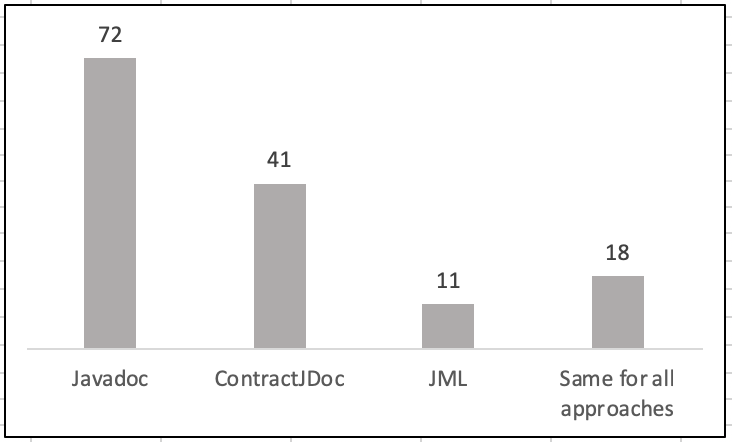
\includegraphics[width=0.7\linewidth]{figs/mostUnderstandable.png}
\label{fig:mostUnderstandable}
\caption{Surveyed Verdicts on the Most Understandable API Documentation Approach.}
\label{fig:surveyResults}
\end{figure}


% individual answers to each approach
After being presented with three versions of the same API, the distribution of assessments for each documentation approach is showed in Figure~\ref{fig:allApproaches}.
%explain visual
Answers for Javadoc and \contractjdoc{} were distributed around a median of $4.0$; for the first, assessments range from $3$ to $5$, while assesments for the latter were no higher than $4$.
Likewise, formal contracts were evaluated with $4$ the highest, however with $3$ with center value. 

\begin{figure}
\centering
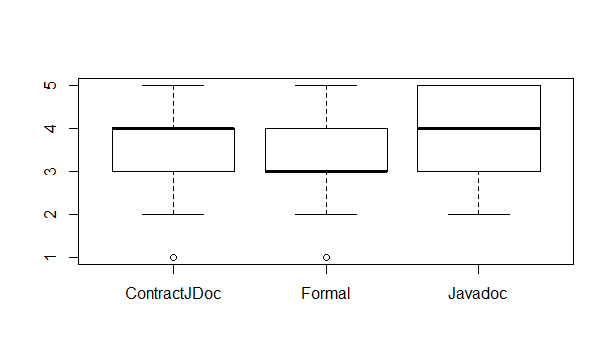
\includegraphics[width=0.7\linewidth]{figs/boxplotApproachesSurveyStudy}
\caption{Surveyed Assessment for Each Documentation Approach.}
\label{fig:surveyResults}
\end{figure}


%statistical results
Differently from the experimental simulation from Section~\ref{sec:expResults}, statistical tests show significant difference between the assessments. The application of One-way ANOVA, which is robust enough for non-normal distributions~\cite{statistical}, detected distinction between the three groups of answers (p-value $<$ 0.05). A corresponding post hoc analysis -- Tukey HSD 
%and pairwise comparisons using t tests
with Bonferroni correction~\cite{statistical} produced the following p-values for each pairwise comparison: Javadoc-ContractJDoc = 0.012, JML-ContractJDoc = 0.000, and JML-Javadoc = 0.000. The results then express significant difference between all approaches.

%When analyzing data grouped by experience (Figures~\ref{fig:javadocExp} to~\ref{fig:jmlExp}) by means of Wilcoxon rank sum test with continuity correctiontests, only for JML we found no statistical difference between Professionals and Students (p-value = 0.17). For both Javadoc and \contractjdoc{}, Professionals had perceived the approaches as being easier for comprehensing than Students (p-value = 0.012 and p-value = 0.004, respectively).


\subsection{Case Study}

Table~\ref{tab:caseStudyResults} exhibits the results of translating real Javadoc specifications to \contractjdoc{} in each system.
%columns
Column \textbf{Faults} presents the failures raised by the original test suite (whose size is showed in Column \textbf{TCs}), with source code enhanced by \contractjdoc{}, while Column \textbf{Time} measures the seconds spent in compiling the system instrumented with \contractjdoc{} before running the test cases. 
%MASSONI: confirmar isso acima.
\textbf{Clauses} displays how many contract clauses were translated into contract expressions, which are classified -- according to XXX et al.~\cite{typeContracts} -- in Columns \textbf{CommCase}, \textbf{AppSpec} and \textbf{Repet}.

\begin{table}
\centering
\caption{Results from Study Replacing Javadoc with \contractjdoc{}.}
\label{tab:caseStudyResults}
\begin{adjustbox}{width=\textwidth}
\begin{tabular}{lrrrrrrr} 
\hline
\multicolumn{1}{l}{\textbf{System}} & \textbf{Faults} & \textbf{Time(s)} & \textbf{TCs}     & \textbf{Clauses}                          & \textbf{CommCase} & \textbf{AppSpec} & \textbf{Repet}  \\ 
\hline
Dishevelled       & 381                                 & 434                                     & 2,643                            & 2,655                                     & 1,536                                  & 151                                    & 968                                   \\
Webprotégé      & 0                                   & 713                                     & 0                                & 930                                       & 717                                    & 282                                    & 1,214                                 \\
ABC-Music-Player  & 2                                   & 14                                      & 30                               & 115                                       & 42                                     & 11                                     & 62                                    \\
Jenerics          & 7                                   & 20                                      & 44                               & 190                                       & 156                                    & 0                                      & 34                                    \\
OOP Aufgabe3      & 1                                   & 4                                       & 11                               & 54                                        & 16                                     & 30                                     & 8                                     \\
%MASSONI: ELIMINEI SimpleShop
% SimpleShop        & 0                                   & 5                                       & 0                                & 50                                        & 30                                     & 11                                     & 9                                     \\
\bottomrule
\textbf{ Total }  & \textbf{391}                      & \textbf{1,185}                        & \textbf{ 2,728 }                 & \textbf{\totalClauses{}} & \textbf{ 2,497 }                       & \textbf{ 282 }                         & \textbf{ 1,214}                       \\
\bottomrule
\end{tabular}
\end{adjustbox}
\end{table}


% \begin{table*}[h]
% \caption{Results from Applying \contractjdoc{} Replacing Javadoc.}
% \label{tab:caseStudyResults}
% \centering
% \begin{tabular}{l l l l l l l l}
% \hline
%  \bfseries System &
%  \bfseries \#Clauses & 
%  \bfseries \#Errors & 
%  \bfseries Time (s) &
%  \bfseries \#Tests &
%  \bfseries \#Com.Case &
%  \bfseries \#AppSpec. &
%  \bfseries \#Repet. \\ \hline
% ABC-Music-Player & 115 & 2 & 14 & 30 & 42 & 11 & 62 \\
% Dishevelled & 2,655 & 381 & 434 & 2,643 & 1,536 & 151 & 968 \\
% Jenerics & 190 & 7 & 20 & 44 & 156 & 0 & 34 \\
% OOP Aufgabe3 & 54 & 1 & 4 & 11 & 16 & 30 & 8 \\
% SimpleShop & 50 & 0 & 5 & 0 & 30 & 11 & 9 \\
% Webprot\'{e}g\'{e} & 930 & 0 & 713 & 0 & 717 & 79 & 133 \\ \hline

%  \bfseries Total & 
%  \bfseries \totalClauses{} & 
%  \bfseries 391 &
%  \bfseries 1,185 &
%  \bfseries 2,728 &
%  \bfseries 2,497 &
%  \bfseries 282 &
%  \bfseries 1,214
% \\
% \bottomrule
% \end{tabular}
% \end{table*}


%commentary on the table
From the selection of open source systems, only \emph{WebProtégé}'s test suites were unavailable; we translated their clauses nonetheless due to the richness of its Javadoc specification.
The size of the available test suites is proportional to the system size.
\emph{Dishevelled} is much larger than the other selected systems, naturally presenting a higher rate of anomalies, which provided us a profuse source of analysis about the mismatches between specification and implementation. 
%MASSONI: temos o tempo que cada sistema usou pra compilar SEM A INSTRUMENTACAO?
About the time...



% results for contract types
Concerning the kind of contracts, the only unit in which we wrote more
application-specific contracts was \emph{OOP Aufgabe3} system (55\% of the
written contracts are application-specific). On the other hand, in \emph{ABC-Music-Player}, more than 90\% of the contracts remains between common-case and repetitive code: verifications that strings are not blank, collections are not empty, or that a method returns a field.
For \emph{Dishevelled}, most contracts are classified as common-case (57.51\%) -- 
%other 36.92\% are repetitive with code and 
only 5.57\% are application-specific.
Similarly, all contracts written for \emph{Jenerics} are related to verification of nullity from parameters or the return value, thus all contracts
remains between common-case and repetitive code.
For \emph{WebProt\'{e}g\'{e}}  common-case contract expressions amount to 77.51\%.  

%In \emph{SimpleShop}, the written contracts are distributed in the following manner: common-case 60\%, repetitive code 19\%, and application-specific 21\%; again the number of common-case and repetitive code outperforms application-specific contracts. 

